\documentclass[11pt]{exam}

% Preamble % (fold)

\usepackage[paper=letterpaper,margin=.75in,twoside=false,includehead]{geometry}

\usepackage{amsfonts,amsmath,amsthm,amssymb} 
\usepackage{enumerate}
\usepackage{graphicx}

\usepackage{paralist}
\usepackage{multicol}


\let\svthefootnote\thefootnote

\newtheorem*{thm}{Theorem}
\newtheorem*{conjecture}{Conjecture}

\newcommand{\Z}{\mathbb{Z}}
\newcommand{\E}{\mathbb{E}}
\newcommand{\N}{\mathbb{N}}
\newcommand{\cP}{\mathcal{P}}
\newcommand{\R}{\mathbb{R}}


\usepackage{tikz, xcolor}

\title{Communicating in Mathematics (MTH 210) Final Exam}
\date{April 22, 2019}


\begin{document}



\maketitle

\noindent Do not start this exam without having read the what to expect document and the following instructions.\\

\noindent The exam is open book and notes.  You may use a calculator or Desmos (or other graphing technology) if you'd like to graph something, but otherwise no technology is allowed. You should not use Blackboard or other internet resources, and no collaboration is allowed. Violation of this policy could result in failure of the course.

\noindent You can print the exam or write answers in your notebook. Either way you will upload a single PDF of your answers on Blackboard. If you write in a notebook, {\bf please start each new page of the exam on a new page in your notebook}.\\

\noindent Carefully read each question and make sure you answer all parts.\\

\noindent Do not panic if you don't know how to answer a question. See the What to Expect document for how to earn partial credit in this case.\\

\noindent You can earn 1/8 of a point for every classmate's (first) name you list on the first page of your exam.






\addpoints

\begin{center}
\gradetable[v]
\end{center}


%\vspace{.3in}

%\begin{center}
%Name (print): \underline{\hspace{3in}}  
%\end{center}


\pagebreak




\begin{questions}

% Definitions and Notation
\question[10] 
	%\begin{parts}
	%\part 
	Complete the definition: ``An integer $a$ is an odd integer provided that...". Then use the definition to explain why $-5$ is odd.

\vfill

%Logic
\question[10]  A mathematician places a set of four cards on a table, each of which has an integer on one side and a colored patch on the other side. She claims the following: 
\begin{center}
\emph{ if a card shows an odd integer on one face, then its opposite face is green}
 \end{center}
 
  The visible faces of the cards show 3, 8, green, and pink. 

\begin{center}
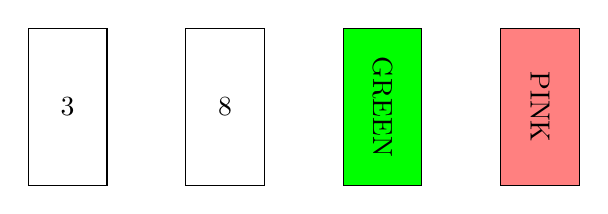
\begin{tikzpicture}
\draw (0,0) rectangle (1,2);
\draw (.5,1) node {$3$};
\draw (2,0) rectangle (3,2);
\draw (2.5,1) node {$8$};
\draw[fill=green] (4,0) rectangle (5,2);
\node[rotate=-90] at (4.5,1)  {GREEN};
\draw[fill=red!50] (6,0) rectangle (7,2);
\node[rotate=-90] at (6.5,1)  {PINK};
\end{tikzpicture} 
\end{center}


Which card(s) \emph{must} you turn over in order to test the truth of her claim?  Use a truth table for ``if $P$ then $Q$" to carefully explain why you must flip over the cards you chose and why you don't have to flip over the other cards.
\vfill
\vfill
\vfill

\newpage


%Proof Techniques What to Assume
\question[10] For both parts of this problem use the following statement:
\begin{center}
For all integers $a$ and $b$ if $5\mid ab$ then $5\mid a$ or $5\mid b$.
\end{center}
	\begin{parts}
	\part State what you would assume in a proof by contrapositive of the statement.
	\vfill
	\part State what you would assume in a proof by contradiction of the statement.
	\vfill
	\end{parts}



%Proof Techniques - which to use
\question[10] Consider the following statement:
\begin{center}
For all $a,b\in\Z$, $ab$ is even if and only if $a$ is even or $b$ is even.
\end{center}
Notice this is a biconditional statement. What two conditional statements do you need to prove?
\vfill

For each, which proof technique would you use and why?
\vfill


\newpage


%Counterexamples
\question[10] Consider the following conjecture:\begin{conjecture}
	For all nonzero integers $k, m,$ and $n$, if $k\mid m$ and $k\mid n$, then $m\mid n$.
	\end{conjecture}
Disprove the conjecture and carefully explain why you know you have shown the conjecture is false.
\vfill


%Proof Critique
\question[10]  Consider the following theorem and proof. 
\begin{thm}
For each $n\in \N$, 
\[1+2+\cdots + n = \frac{n^2+n+1}{2}.\]
\end{thm}
\begin{proof}
We'll use a proof by mathematical induction. Let $P(n) = 1+2+\cdots + n = \dfrac{n^2+n+1}{2}$. We assume that $P(k)$ is true and will show that $P(k+1)$ is true. So,
\[P(k) = 1+2 + \cdots + k = \frac{k^2+k+1}{2}\]
and
\[P(k+1) = 1+2+\cdots + (k+1) = \frac{(k+1)^2 + (k+1) + 1}{2}.\]
By subtracting $(k+1)$ from both sides of $P(k+1)$ we find,
	\begin{align*}
	1+ 2 + \cdots + k + (k+1)&= \frac{(k+1)^2 + (k+1) + 1}{2}\\
	1+2 + \cdots + k &= \frac{k^2+2k+1+k+1+1}{2} - (k+1)\\
	1+2+\cdots + k &= \frac{k^2+3k+3}{2} - \frac{2k+2}{2}\\
	1+2 + \cdots + k & = \frac{k^2+k+1}{2}.
	\end{align*}
So whenever $P(k)$ is true then $P(k+1)$ is true. By the Principle of Mathematical induction, our theorem is true.
\end{proof}

There are many flaws with this proof, identify at least two substantial ones.
\vfill

\newpage

%Sets
\question[10] Let $C = \{c\in \Z \mid c\equiv 0 \pmod{6}\}$ and $D = \{d\in \Z \mid d\equiv 0\pmod{3}\}$. Show that $C\subseteq D$.  (You do not need to write in complete sentences, but your answer should be ``proof like" in that it has all of the key details.)
\vfill

%Functions
\question[10] Let $A = \{a,b,c,d\}$ and $B= \{s,t,u,v\}$. Draw an arrow diagram of $f: A\to B$ so that
	\begin{itemize}
	\item $f$ is a function
	\item the range of $f$ is $\{u,v\}$
	\item a preimage of $v$ is $b$
	\item an image of $a$ is $u$
	\end{itemize}
\vfill

%Equivalence Relations
\question[10] For $(w,x)$ and $(y,z)$ in $\Z\times \Z$ define $(w,x)\sim (y,z)$ if and only if $w\leq y$ and $x\leq z$. Is $\sim$ reflexive? Symmetric? Transitive? Explain using definitions.
\vfill

\newpage

%Proof
\question[10] Prove the following theorem:
\begin{thm}
Let $g: \R\times\R\to \R$ by $g(a,b) = a$. Then $g$ is a surjection and not an injection.
\end{thm}

You should write a formal proof that meets our writing guidelines. Make sure you include a theorem statement!


\vfill



\question\emph{Bonus, up to 5 points:} Write one mathematical thing you learned in MTH 210 that was not covered on this exam.
%\vfill

\end{questions}

\end{document}